\noindent ChatGPT and the realm of search engine AI's were particularly useful in this research process for identifying the different types of technologies currently available, given the market observable on the internet. However, the LLM tended to struggle with providing accurate and specifications from datasheets, requiring the researchers to sift through and locate them. Additionally, ChatGPT was useful for preparing references for sources, but even in this it sometimes struggled to gather the correct article or paper title, although it was strong in being able to provide them in most formats including the IEEE reference style.\\

\subsection{Example 1: Sonar vs. LiDAR}
\noindent One specific example of ChatGPT aiding the research process is by providing a concise explanation of the comparison between the Sonar and LiDAR sensing methods. It is able to be objective and pull from all knowledge of these technologies to best inform our decisions.\\
\begin{figure}[H]
	\centering
	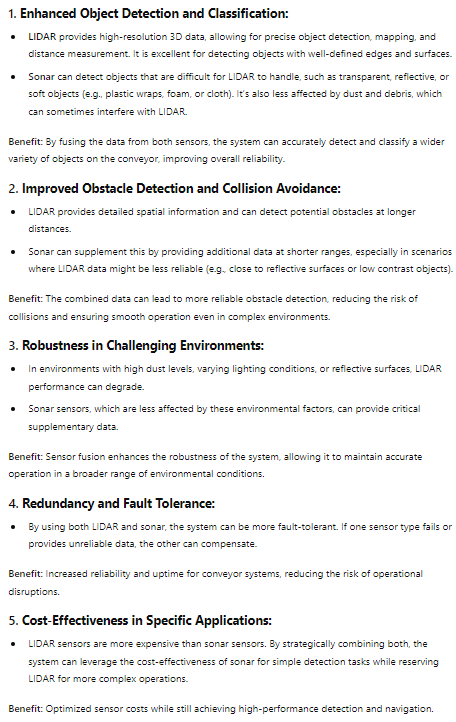
\includegraphics[width=0.5\textwidth]{./Images/chatgpt1.png}
	\caption{\label{fig:chatgpt1}ChatGPT compares sensing technologies}
\end{figure}

% NEED TO CITE CHATGPT

\subsection{Example 2: }

\subsection{Example 3: }